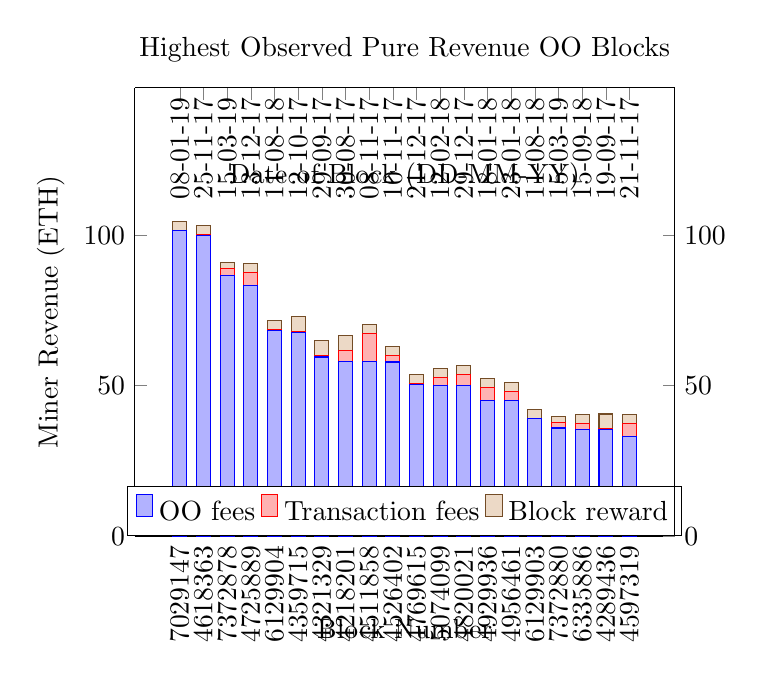
\begin{tikzpicture}
\begin{axis}[
    ybar stacked,
    bar width=5pt,
    ymin=0, ymax=149,
    legend style={at={(0.5,0)},
      anchor=south,legend columns=-1},
          xtick=data,
        x label style={
    at={(0.5,-.25)},
    anchor=south,
},
    ylabel={Miner Revenue (ETH)},
    xlabel={Block Number},
    title={Highest Observed Pure Revenue OO Blocks},
    symbolic x coords={7029147, 4618363, 7372878, 4725889, 6129904, 4359715, 4321329, 4218201, 4511858, 4526402, 4769615, 5074099, 4820021, 4929936, 4956461, 6129903, 7372880, 6335886, 4289436, 4597319, },
    xtick=data,
    x tick label style={rotate=90,anchor=east, at={(axis description cs:0.5,-4.1)}},
      axis y line*=left,
      axis x line*=bottom
    ]
\addplot+[ybar] plot coordinates {(7029147, 101.59262742592085) (4618363, 99.99999999910933) (7372878, 86.5121832) (4725889, 83.4136428437622) (6129904, 68.49918638712944) (4359715, 67.61327299999999) (4321329, 59.567595240292775) (4218201, 58.0644545028598) (4511858, 57.92863275000001) (4526402, 57.900954944999995) (4769615, 50.48518124961362) (5074099, 49.99715453337096) (4820021, 49.9455756) (4929936, 45.12279620448) (4956461, 45.065462) (6129903, 39.166612487152236) (7372880, 35.96297207421013) (6335886, 35.5276) (4289436, 35.4804) (4597319, 33.100512) };
\addplot+[ybar] plot coordinates {(7029147, 0.022575947652901183) (4618363, 0.37137142620000024) (7372878, 2.3880345276524992) (4725889, 4.281388080429975) (6129904, 0.043478875041119955) (4359715, 0.5285118109871835) (4321329, 0.36483124409254397) (4218201, 3.7654935693258866) (4511858, 9.53601230737791) (4526402, 2.0243883310000004) (4769615, 0.34298219062115803) (5074099, 2.720158228981349) (4820021, 3.799417844730175) (4929936, 4.256290607017646) (4956461, 3.0070182564024783) (6129903, 0.050692708979768596) (7372880, 1.8197112616186384) (6335886, 2.0335207370366497) (4289436, 0.14780711818369202) (4597319, 4.267211257) };
\addplot+[ybar] plot coordinates {(7029147, 3) (4618363, 3) (7372878, 2) (4725889, 3) (6129904, 3) (4359715, 5) (4321329, 5) (4218201, 5) (4511858, 3) (4526402, 3) (4769615, 3) (5074099, 3) (4820021, 3) (4929936, 3) (4956461, 3) (6129903, 3) (7372880, 2) (6335886, 3) (4289436, 5) (4597319, 3) };
\legend{\strut OO fees, \strut Transaction fees, \strut Block reward}
\end{axis}

\begin{axis}[
    ybar stacked,
    bar width=5pt,
    ymin=0, ymax=149,
    symbolic x coords={08-01-19, 25-11-17, 15-03-19, 13-12-17, 11-08-18, 12-10-17, 29-09-17, 30-08-17, 08-11-17, 10-11-17, 21-12-17, 12-02-18, 29-12-17, 18-01-18, 23-01-18, 11-08-18 , 15-03-19 , 15-09-18, 19-09-17, 21-11-17, },
    xlabel={Date of Block (DD-MM-YY)},
    xtick=data,
        x label style={
    %at={(0.5,1.065)},
    at={(0.5,.75)},
    anchor=south,
},
    x tick label style={rotate=90,anchor=east},
      axis y line*=right,
      axis x line*=top,
    ]
    \addplot+[ybar] plot coordinates {(08-01-19, 0) (25-11-17, 0) (15-03-19, 0) (13-12-17, 0) (11-08-18, 0) (12-10-17, 0) (29-09-17, 0) (30-08-17, 0) (08-11-17, 0) (10-11-17, 0) (21-12-17, 0) (12-02-18, 0) (29-12-17, 0) (18-01-18, 0) (23-01-18, 0) (11-08-18 , 0) (15-03-19 , 0) (15-09-18, 0) (19-09-17, 0) (21-11-17, 0) };

\end{axis}


\end{tikzpicture}


